\section{Objective}
\label{sec:Obj}
The objective of this experiment is the understand the workings of a silicone strip detector and its properties. Additionally the use of the readout electronics and resulting data is supposed to further introduce the participant into their usage in different detector systems.
\section{Theory}
\label{sec:Theo}

In order to understand a silicone strip detector it is important to look at theory of semiconductors.
\subsection{Semiconductors}
Semiconductors are defined by the energy gap of the valence and conduction band. If the bands overlap in a material it is referred to as \textit{conductor} since the electrons can move freely in the material. If the energy gap is to great the electrons can't travel into the conduction band, therefore these materials are called \textit{insulators}. If though the energy gap is in the range below \qty{3}{\eV} the material is a \textit{semiconductor}. The semiconductor employed in this experiment is silicone with a band gap of \qty{1.107}{\eV} \cite{lab}. Silicone has four valence electrons and arranges itself in a diamond lattice structure. One of the properties of a semiconductor is, if the valence electrons are exited e.g. thermal effects or other external particles, it creates a hole in the valence band, which can be treated as a quasi particle with a negative charge. The electron and hole can form a bound state resembling an atom, if the material is placed into a electric field (e.g. by placing a cathode/anode to the materiel) the formation of such a state is prevented. The electrons and holes can now travel th the cathode/anode. This behavior can be modified be a process called \textit{doping}, in which some of the silicone particles in the crystalline structure are replaced by elements that carry a higher/lower amount of valence electrons. %auch noch bild einfuegen

\subsubsection{n-type semiconductor}

If the element, used for doping, has a valence charge higher than four (e.g. Arsenic: five valence electrons) one electron is not used for the binding in the crystalline structure so it can move basically freely in the material. 

\subsubsection{p-type semiconductor}
Analog to the n-type semiconductor the introduced material has fewer electrons in its valence band (Boron: three valence electrons). The boron would then leave one of the bonds to the it surrounding silicone atoms partially empty creating a hole, which then can move freely like the electron. 


\begin{figure}
	\centering
	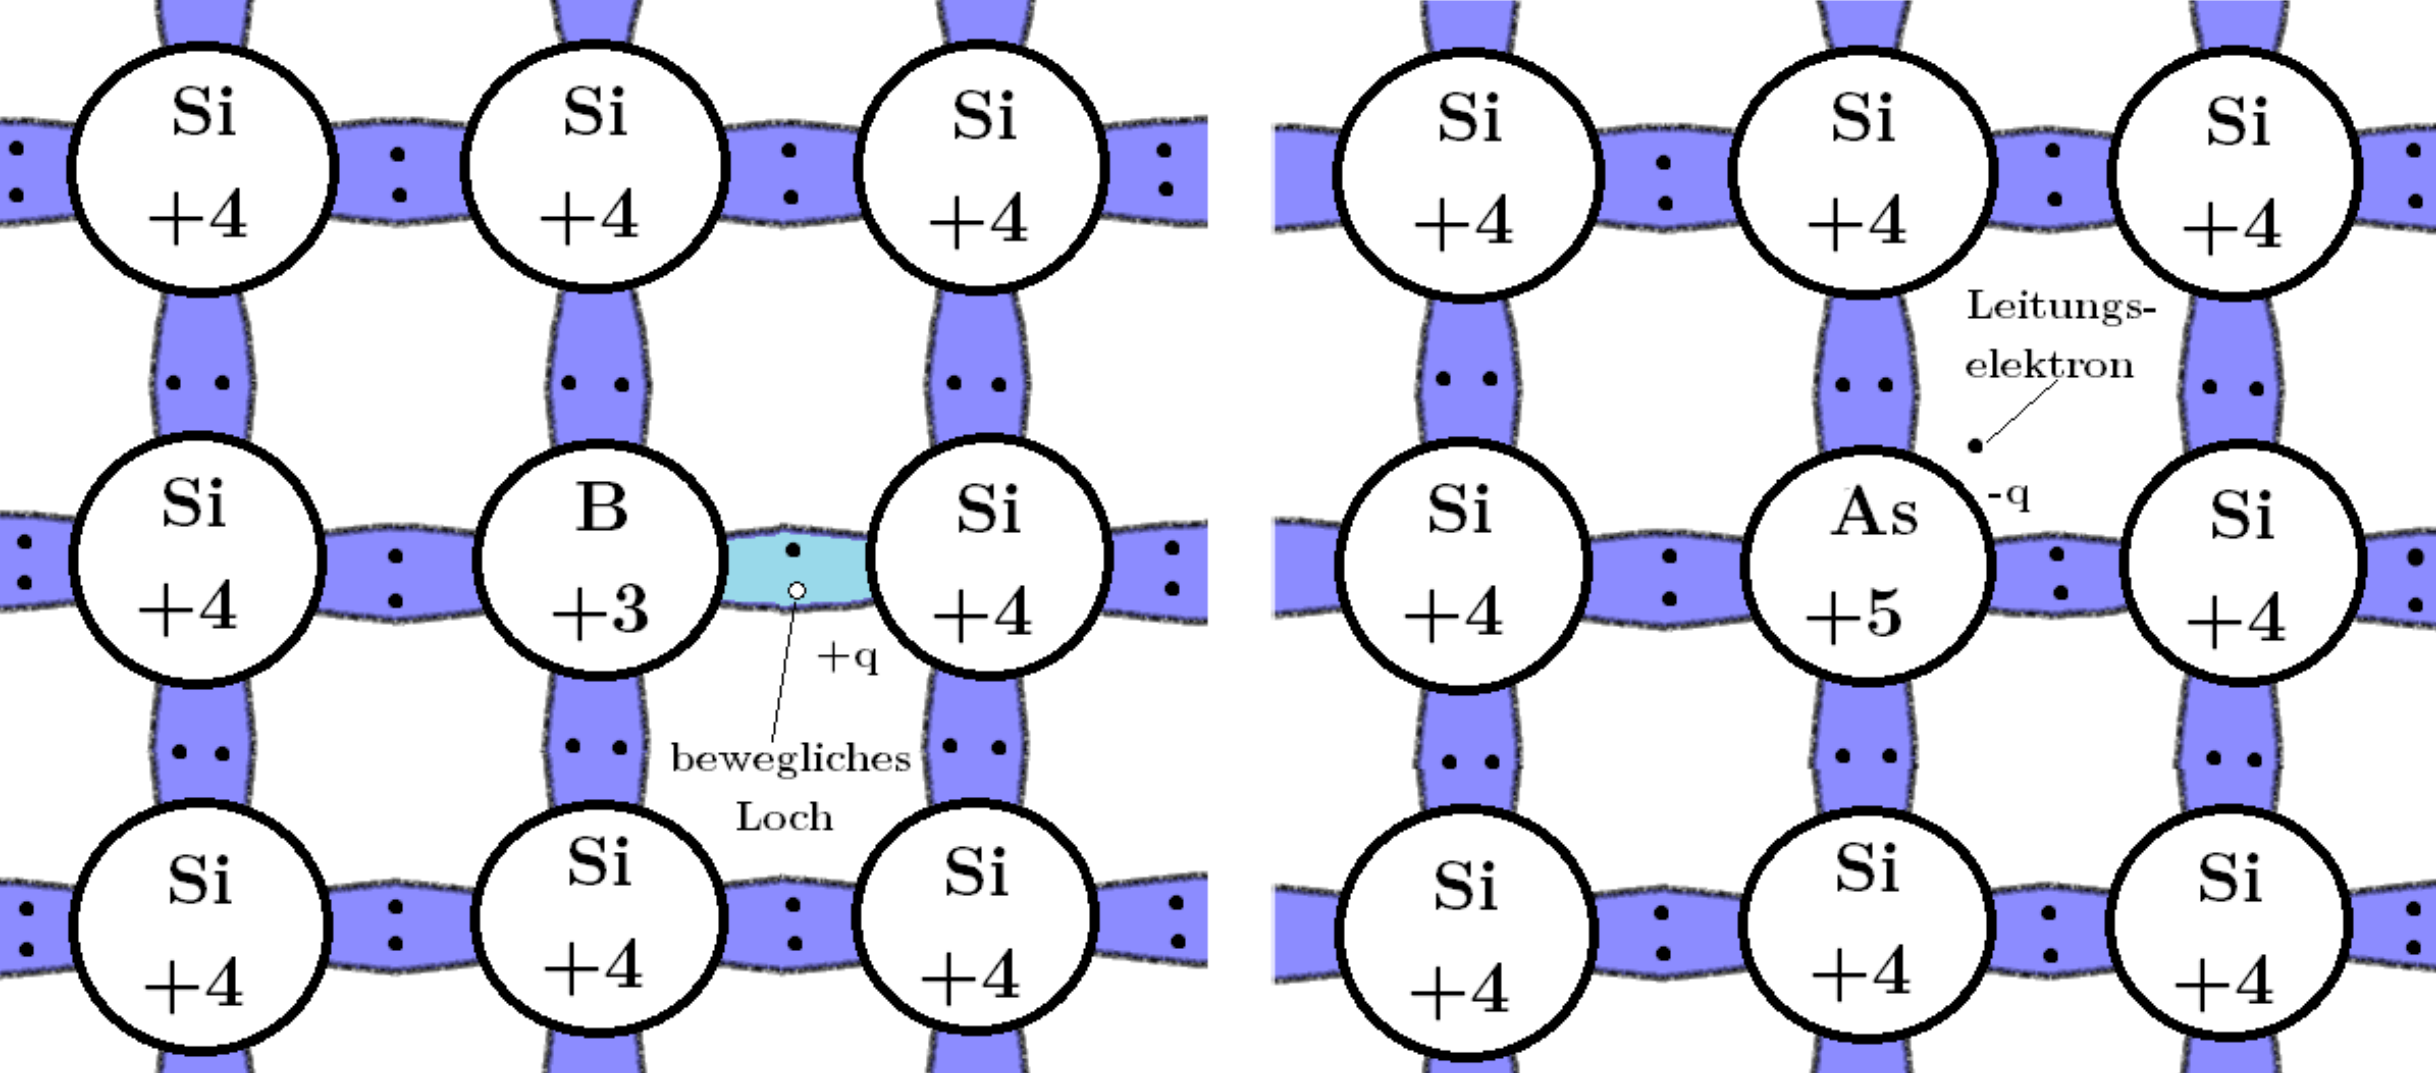
\includegraphics[width=0.7\linewidth]{Assets/doting.png}
	\caption{graphical representation of boron and arsenic doping in silicone\cite{lab}.}
	\label{fig:doting}
\end{figure}


\subsubsection{pn transition}
If one connects a p and n doped material together a diode is created.% This pn transition is the bas
Inside the diode the additional electrons from the n-side now want to recombine with the holes from the p-side. This results in a positive charge on the n-side and a negative on the p-side. The resulting difference of a few \unit{\milli\volt} is called diffusion voltage $U_\mathrm{D}$ \cite{lab}. \\

For the Detection of ionizing particles a voltage is applied to either side of the diode, the electrons from coming from the applied potential are then recombining with the holes on the p-side and the electron in the n-side flow into the anode, resulting in a zone in which no free charge carriers remain. This zone is called the \textit{Depletion zone} and its dimension can be determined to be
\begin{equation}
	d(U) = \sqrt{\frac{2\epsilon(U_\mathrm{D}+ U)}{eN_\mathrm{eff}}},
	\label{depl}
\end{equation}
where U is the voltage applied to the diode, $\epsilon$ the dielectric constant of silicone, $e$ the elementary charge and $N_\mathrm{eff}$ the effective charge carrier density. $N_\mathrm{eff}$ is determined by 
\begin{equation}
	N_\mathrm{eff} = \frac{N_\mathrm{D}N_\mathrm{A}}{N_\mathrm{D}+N_\mathrm{A}},
\end{equation}
where $N_\mathrm{D}$,$N_\mathrm{A}$ are the respective densities of the n and p doped materials. When the depletion zone is as large as the diode itself, one speaks of a full depletion at the depletion voltage $U_\mathrm{dep}$. Using the fact that $U\ll U_\mathrm{D}$ it can be determined that $u_\mathrm{dep}$ is given by
\begin{equation}
	U_\mathrm{dep} \approx \frac{e}{2\epsilon} N_\mathrm{eff} D^2
\end{equation}
with the thickness of the diode $D$. If the applied voltage is below the depletion voltage then the distance $d_\mathrm{c}(U)$ can be approximated with

\begin{equation}
	d_\mathrm{c}(U)= D\sqrt{\frac{U}{U_\mathrm{depl}}}.
\end{equation}
Ideally the diode is fully depleted so the signal generated by an ionizing particle can be detected. This is not the case since thermal effects an electron can enter the current band and create the so called \textit{leakage current}. This effect increases with higher voltages. The relation between the current and voltage can be seen in \autoref{fig:leackage}.

\begin{figure}
	\centering
	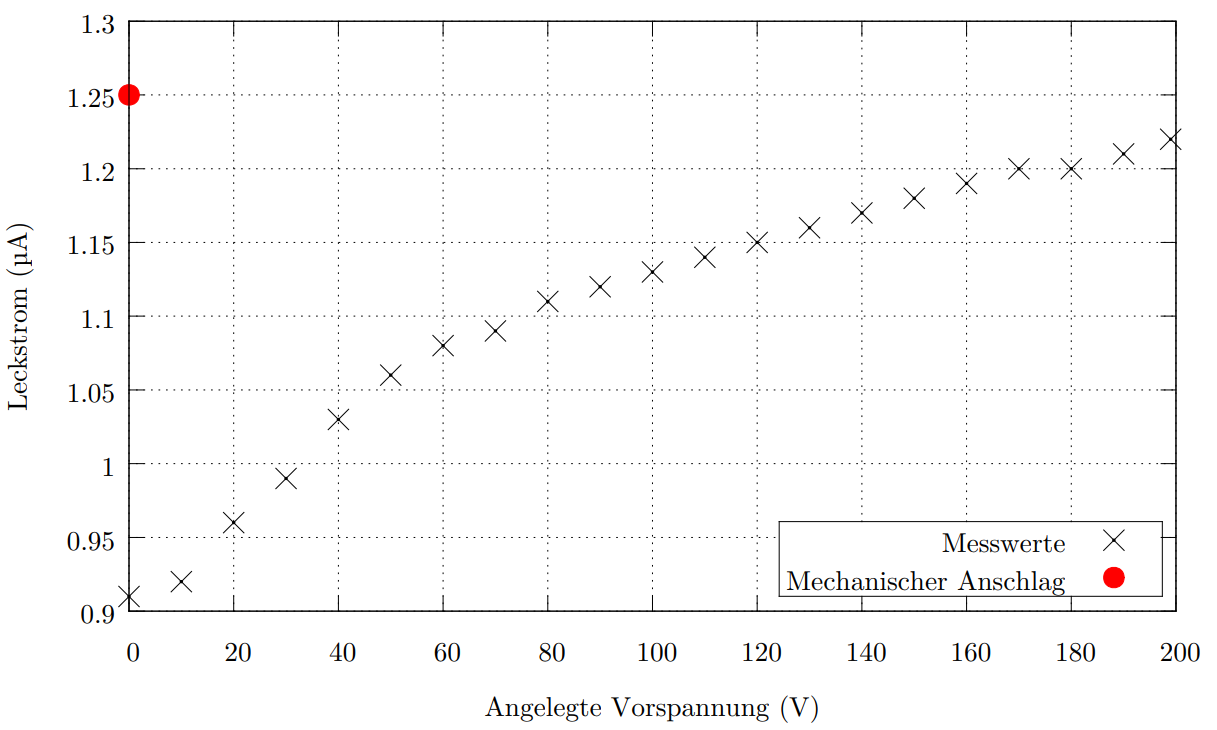
\includegraphics[width=0.7\linewidth]{Assets/leackage}
	\caption{Current measured across the sensor in relation to the applied voltage \cite{lab}.}
	\label{fig:leackage}
\end{figure}


Using this plot the depletion voltage can be determined as the voltage at which the leakage current only increases linearly.

\subsection{Ionizing radiation}
The silicone strip detector sets out to detect ionized particles. During the experiment a source producing beta particles is employed.
\subsubsection{Beta decay}
The used source is the strontium isotope \ce{^{90}Sr}, which decays via a $\beta^-$ decay into yttrium (maximal energy \qty{0.545}{\mega\eV}), that intern decays into zirconium (maximal energy \qty{2.28}{\mega\eV}) \cite{lab}.
\begin{equation}
	\ce{^{90}Sr} \rightarrow \ce{^{90}Y} \rightarrow \ce{^{90}Zr}
\end{equation}

During a $\beta^-$ decay a neutron in the atomic nucleus decays into a proton, electron and an anti-electron-neutrino. Since this process is a three body decay the electron is nor produced at a fixed energy. The energy of the emitted electron follows the distribution shown in \autoref{}


\begin{figure}
	\centering
	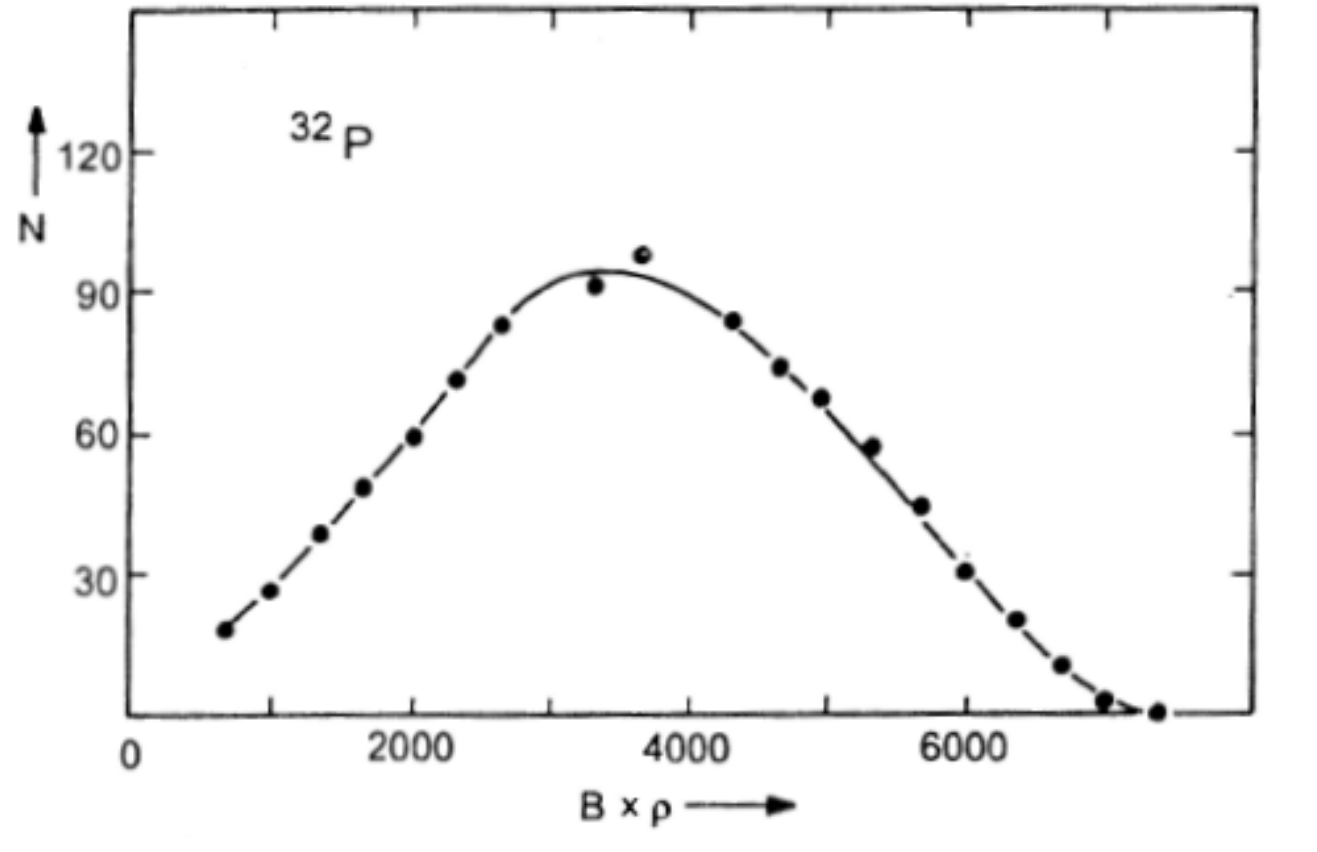
\includegraphics[width=0.7\linewidth]{Assets/edist.png}
	\caption{Energy distribution of a electron originating from ab $\beta^-$ Decay \cite{lab}.}
	\label{fig:edist}
\end{figure}

The activity is defined as the rate of change of the number of nuclei $A = - \dot{N}$. From this it can be deduced that the activity can be written as

\begin{equation}
	A = \lambda N_0 \exp(-\lambda t) = A_0 \exp(-\lambda t),
\end{equation}
where $A_0$ and $N_0$ are the activity and number of nuclei at $t=0$, and $\lambda$ is the decay constant of the decaying material/particle.

\subsubsection{Interaction in matter}
Due to the energy of the electrons almost only their collisions with the nuclei in the it traversing matter are contributing to the energy loss. The ionizing particles inside the detector are detected by these collision, as they excite the electrons in the crystalline structure of the detector material. These exited electron then create a measurable signature in the detector. The energy deposited by the electrons can be determined using the Bethe-Bloch equation with additional correction therms:
\begin{equation}
	-\frac{\mathrm{dE}}{\mathrm{d}x} = 2\pi N_{\mathrm{a}} m_e c \rho \frac{Z}{A} \frac{1}{\beta^2} \left[ln\left(\frac{\tau(\tau+2)}{2(I/m_ec^2)^2}\right)+F(\tau) - \delta - 2\frac{C}{Z}\right],
\end{equation}
with 
\begin{equation}
	F(\tau) = 1 - \beta^2 + \frac{\frac{\tau}{8}+(2r_e +1 )\ln(2)}{(\tau+1)^2}, \hspace{0.5cm} \mathrm{where}\hspace{0.2cm} \tau = \gamma-1.
\end{equation}
The meaning of the symbols and their values can be seen in \cite{lab}.
From this formula it can be determined that the electron originating from the \ce{^{90}Sr} source is depositing \qty{3.88}{\mega\eV} per \unit{\centi\meter} \cite{lab}.\\

Usually for particles traversing a silicone detector the deposited energy can be approximated by a Gaussian distribution. As for a thinner detector (e.g. like the \qty{300}{\micro\meter} of the detector used in this experiment) the thickness is not sufficient enough for the energy loss to be described as Gaussian. The actual distribution is much better described by a Landau distribution. Another effect at play steam from the already described energy distribution of the emitted electron. This results in a convoluted Landau distribution shown in \autoref{fig:landau}.


\begin{figure}
	\centering
	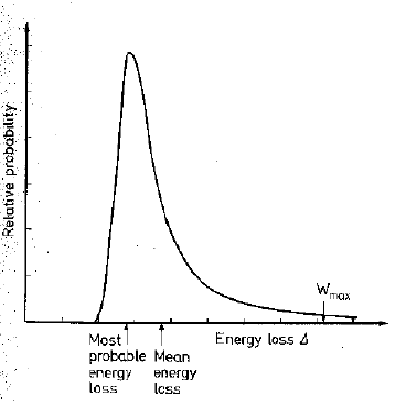
\includegraphics[width=0.45\linewidth]{Assets/landau}
	\caption{Convoluted Landau distribution \cite{lab}.}
	\label{fig:landau}
\end{figure}


\subsection{Noise and pedestals}
As most electronics and detectors can't operate a hundred percent clean, there will always remain noise, signals that interfere with the intended measurement. So the recorded counts from the Analog-Digital-Converter (ADC) can be described by

\begin{equation}
	\mathrm{ADC}(i,k) = \mathrm{P}(i) + \mathrm{D}(k) + \mathrm{Signal}(i,k),
\end{equation}
ADC is the probability for a signal $k$ at the $i$-th strip on the detector. $\mathrm{P}(i)$ is the so called \textit{pedestal}. It is determined as the mean value of the $\mathrm{ADC}(i,k)$ without $\mathrm{Signal}(i,k)$. So $\mathrm{P}(i)$ calculated for $N$ measurements as 
\begin{equation}
	\mathrm{P}(i) = \frac{1}{N} \sum_{k=1}^{N}\mathrm{ADC}(i,k).
\end{equation}
The $\mathrm{D}(k)$ contribution is the \textit{common mode shift} and is calculated using 
\begin{equation}
	\mathrm{D}(k) = \frac{1}{128}\sum_{i=1}^{128}(\mathrm{ADC}(i,k) - \mathrm{P}(i))
\end{equation}
From these distributions using the root mean square the noise is determined:
\begin{equation}
	\mathrm{Noise}(i)=\sqrt{\frac{1}{N-1}\sum_{k=1}^{N}(\mathrm{ADC}(i,k) - \mathrm{P}(i) - \mathrm{D}(k))^2}
\end{equation}